\section{Competitive options enter bargaining, but do not identify a price premium}
\label{sec:bargain}

\subsection{Completion and rejection depend on who responds and when}

Across 526 threads, the agents accept 113 offers, counter 394, and reject 413. No trade response is a deterministic fallback. The four configurations accept similar absolute numbers, twenty-six to thirty each, while their alternatives to agreement differ. Sol counters 140 of 235 received offers and Opus 141 of 189. Gemini rejects 180 of 242 and Grok 149 of 254. Opus's response path is action-only recovery in 162 responses. Similar acceptance totals therefore coexist with very different interaction histories.

\begin{table}[t]
\centering\small
\begin{tabular}{@{}lrrr@{}}\toprule
Offer completes & All, A/C/R & Opening, A/C/R & Later, A/C/R\\\midrule
Author only & 19/111/159 & 3/46/138 & 16/65/21\\
Recipient only & 24/78/38 & 2/18/31 & 22/60/7\\
Both & 10/35/36 & 3/11/34 & 7/24/2\\
Neither & 60/169/179 & 24/62/152 & 36/107/27\\\midrule
All & 113/393/412 & 32/137/355 & 81/256/57\\\bottomrule
\end{tabular}
\caption{Acceptance-legal offers only, $N=918$. A/C/R denote accept, counter, and reject. Two additional ineligible openings receive one counter and one rejection. Later offers are selected continuations.}
\label{tab:responses}
\end{table}

The pooled rejection rate is 55.0\% when only the author completes and 27.1\% when only the recipient completes. Separating thread position reduces the difference from 27.9 percentage points to 13.0 for openings and 12.7 for later offers. Author-only offers disproportionately open threads, where rejection is common. Joint recipient-by-stage cells further qualify the pattern. Its rejection ordering holds in five of six Sol/Gemini/Grok cells; Opus reverses the pooled comparison, rejecting 3/52 author-only and 6/42 recipient-only offers. Appendix~\ref{app:joint} preserves all cells, including small denominators. These distributions establish varied responses to heterogeneous transactions, rather than a controlled preference for denying completion.

The reasons are more specific than the response categories. Among thirty-eight outright refusals of recipient-only completion, both inherited readings identify a stated rival consequence in twenty-seven. The corresponding count is thirty-four of thirty-six when both sides complete. The recipient-only cases matter because no rival group is newly completed by that transaction. Cash, retained blockers, and other holdings can still improve a rival's competitive position. However, thirty-four common-positive labels come from G1 and G15, and all eight Opus records lack private notes. This is concentrated evidence of explicit considerations, not a comparison of underlying reasoning ability.

\subsection{Generic repricing and mixed within-deed evidence}

Counters often demand more cash without changing the property exchange. Of 111 counters to author-only completion offers, ninety-two preserve all requested deeds, and seventy-nine preserve the entire noncash bundle while improving the counterer's cash. In the comparison population of 110 non-completing offers requesting a deed, eighty-seven preserve all requested deeds and eighty-one preserve the noncash bundle while improving cash. Sol and Opus supply most counters in both populations. Repricing is therefore a broad bargaining practice. Its occurrence alone cannot establish that an agent priced a rival's development opportunity.

Seller asks show more consistent aggregate ordering than buyer bids. For unmortgaged deeds, median asks divided by list price are 2.81 versus 2.00 for Sol, 2.00 versus 1.50 for Opus, and 4.14 versus 1.82 for Grok, comparing recipient completion with neither-party completion. Mortgaged asks have the same ordering for these three sellers. Jointly separating seller, mortgage status, and opening versus later position gives eleven higher completing asks and one reversal among their twelve populated comparison cells. The reversal is Opus's unmortgaged later offers, with medians 1.86 versus 2.10. Gemini has too few asks for a useful profile. Full cells and exact sample sizes appear in the appendix.

These aggregate comparisons still combine different deeds. Only seven game/seller/single-deed groups contain asks to both completing and non-completing buyers. Four have higher median asks to the completing buyer, two lower, and one equal, as shown in Figure~\ref{fig:prices}. Requiring the same mortgage status and thread position leaves five comparison cells: three higher, one lower, and one equal. The strongest available restrictions thus preserve counterexamples and sharply reduce overlap. We do not label the unmatched ordering a seller premium, an endowment effect, or an efficient response to externalities. Buyer bids also change ordering across configurations and cuts, preventing a general claim that only sellers recognize completion value.

\begin{figure}[t]
\centering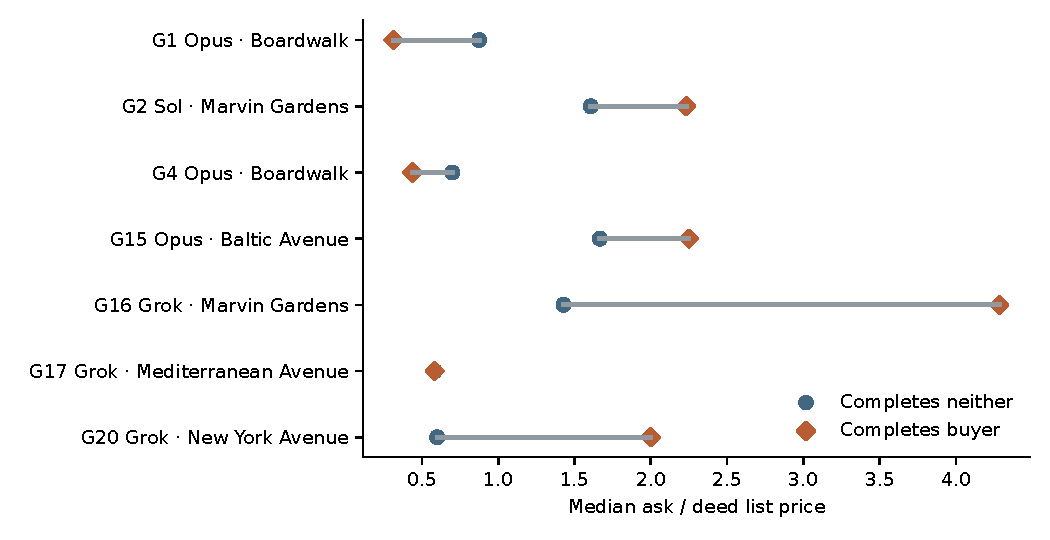
\includegraphics[width=\linewidth]{same_deed.pdf}
\caption{Every game/seller/single-deed group containing both kinds of seller ask. Points are within-group median asking cash divided by that deed's list price. Four lines rise toward the completing buyer, two fall, and one ties. Buyers, dates, and negotiations differ. Mortgage and stage restrictions reduce the overlap to five cells, reported in Appendix~\ref{app:prices}.}
\label{fig:prices}
\end{figure}

\Incident{g2}{A blocker is priced through construction and resale}

At G2 turn 45, Opus holds two yellows and bids \$325 for Sol's Marvin Gardens. Sol's public demand and attached note link the price to the rival's development budget:
\TranscriptQuote{g2-d124-price}
\TranscriptQuote{g2-d124-note}
One turn earlier, Sol asked Grok \$450 for the same deed after a \$200 bid. Grok owned no yellow, but Sol's earlier note explicitly considered Grok reselling it to Opus. The non-completing buyer is already a potential intermediary in the seller's account. The later ask of \$650, then \$600, therefore concerns a competitive network, not merely a bilateral change in set status.

Sol correctly calculates the \$520 residual cash but incorrectly says it buys nine yellow houses. At \$150 per house it buys three. House costs are absent from this current prompt. The error limits the numerical valuation without erasing the stated concern. Opus publicly calls \$450 final while its private note allows roughly \$475. Sol refuses. At turn 69 the roles reverse: cash-poor Opus, now holding \$17, gives its two yellows for Sol's two railroads plus \$100. Sol completes yellow, spends \$300 on houses, receives \$150 salvage and \$44 undeveloped rent, but no developed yellow rent. The yellows eventually reach Gemini through bankruptcy. Competitive attention is clear; the later history does not validate either ask.
\Source{G2 d119--128 and d197--198; exact-field definitions inherited from the integrated Opus manifest. G2 rent event 1566 distinguishes undeveloped rent from developed receipts.}

\Incident{g15}{A recipient refuses its own completion after revised terms}

At G15 turn 63, Sol has \$730 and Grok \$333. Sol offers its two greens for Grok's Ventnor plus \$100, completing both sides. Grok's note evaluates the relative construction budgets:
\TranscriptQuote{fx-g15-refusal-note}
The balances of approximately \$830 and \$233 agree with the ledger. A full first green layer costs \$600, but a single legal house costs \$200. The note concerns a full layer rather than the minimum available investment. Sol removes its cash request, adds Kentucky, and finally offers cash:
\TranscriptQuote{fx-g15-sweetener}
\TranscriptQuote{fx-g15-final-refusal}
No deal settles. Grok is eliminated eighteen turns later and its blockers pass to Gemini; Sol never completes yellow or green. This exchange provides stronger evidence of responsiveness than a bare strategic phrase: the proposer addresses a stated objection, and the recipient maintains a refusal tied to timing and rival finance. It supplies no reference continuation establishing whether refusal or agreement would have been better.
\Source{G15 d168--175, standard responses. Cash balances are offer-ledger arithmetic; public-message delivery is checked against the counterparties' actual requests.}

\subsection{Public claims, corrections, and agreement}

The complete response census does not reveal whether accepting a deal means endorsing its explanation. Two cases show why that distinction matters. The first contains an explicit public limit below a private contingency. The second contains a false board premise corrected by the recipient while the exchange executes. They place communication in its bargaining role without measuring a persuasion effect.

\Incident{g7}{A public final price below a private contingency settles}

Sol asks \$625 for North Carolina. Grok replies with a lower public limit while retaining a higher private contingency:
\TranscriptQuote{g7_d42_public}
\TranscriptQuote{g7_d42_private}
\TranscriptQuote{g7_d43_public}
Sol's note favors reinvestment over waiting for another \$25. The contradiction between the advertised final price and the same-response contingency supports a bargaining-bluff interpretation under a prompt that permits it. Agreement establishes the settled price, not that the bluff caused Sol's concession. Grok later completes green through an auction at turn 95, never builds it, and loses its estate to Sol at turn 110. Sol develops the inherited group two turns later. The same deed can thus pass through purchase, negotiated resale, and creditor acquisition without its initial negotiation determining the eventual productive owner.
\Source{G7 d41--43; auction event 1680, estate events 1946--1954, build events 1971--1973.}

\Incident{g19}{The recipient corrects the premise and accepts the terms}

Grok's received call proposes Virginia and \$150 for States, falsely describing States as orange. The same response's note says it has misread the board and should abort. Sol receives the false message but answers:
\TranscriptQuote{g19_d135_false_public}
\TranscriptQuote{g19_d136_correction_accept}
The swap executes and completes neither group. Sol's note calls the terms strictly favorable. Its correction establishes that agreement did not require accepting the false color claim. Grok's content names \End{} while its received call proposes the swap; the public message supports the call. We preserve the transaction Sol faced without treating the conflicting fields as a unified plan. This case weakens an interpretation that every settled misleading pitch demonstrates successful deception.
\Source{G19 d135--136, standard first attempts. Current holdings confirm both deeds are pink; the false message is present in Sol's delivered request.}

\subsection{Who supplies construction finance?}

Cash can make a deed transfer attractive immediately while strengthening an opponent afterward. Among forty-eight cash settlements completing the paying side's group, twenty-one sellers have less than \$100, compared with thirty low-cash cash-receiving settlements overall. Opus supplies thirteen of those twenty-one. Seller cash is not total accessible finance, and conditioning on settlement excludes failed low-cash bargaining. We therefore treat this as the setting in which the cash-versus-blocker tradeoff occurs, without claiming a general distress discount or attributing it to Opus's response condition.

\Incident{g20}{An appeal to deny construction funds receives mixed participation}

Opus sells Illinois to Grok for \$500, completing reds and leaving Grok \$222. A red house costs \$150. Gemini addresses the table:
\TranscriptQuote{g20-coordination-appeal}
Grok's next selected note recognizes the appeal as a cash boycott. Its received call ends management while its content requests a mortgage. Later, Grok offers Vermont to Gemini for \$150. Gemini refuses:
\TranscriptQuote{g20-concrete-refusal}
Grok mortgages Vermont for \$50 instead. Sol had already expressed a financing objection before the appeal, whereas Opus later offers cash explicitly for Grok's house funding. Neither Opus offer settles. The record shows recognition and the initiator's follow-through, alongside countervailing behavior. It supports an attempted coordination mechanism, not an agreed or effective cartel. Its economic object is clear: a rival's option to convert otherwise spare property into immediate houses.
\Source{G20 d95--102, d129--130 and d156--160. The appeal appears in Grok's d97 request; recognition is selected attempt 1.}
